% Options for packages loaded elsewhere
\PassOptionsToPackage{unicode}{hyperref}
\PassOptionsToPackage{hyphens}{url}
%
\documentclass[
]{ltjarticle}
\usepackage{lmodern}
\usepackage{amssymb,amsmath}
\usepackage{ifxetex,ifluatex}
\ifnum 0\ifxetex 1\fi\ifluatex 1\fi=0 % if pdftex
  \usepackage[T1]{fontenc}
  \usepackage[utf8]{inputenc}
  \usepackage{textcomp} % provide euro and other symbols
\else % if luatex or xetex
  \usepackage{unicode-math}
  \defaultfontfeatures{Scale=MatchLowercase}
  \defaultfontfeatures[\rmfamily]{Ligatures=TeX,Scale=1}
\fi
% Use upquote if available, for straight quotes in verbatim environments
\IfFileExists{upquote.sty}{\usepackage{upquote}}{}
\IfFileExists{microtype.sty}{% use microtype if available
  \usepackage[]{microtype}
  \UseMicrotypeSet[protrusion]{basicmath} % disable protrusion for tt fonts
}{}
\makeatletter
\@ifundefined{KOMAClassName}{% if non-KOMA class
  \IfFileExists{parskip.sty}{%
    \usepackage{parskip}
  }{% else
    \setlength{\parindent}{0pt}
    \setlength{\parskip}{6pt plus 2pt minus 1pt}}
}{% if KOMA class
  \KOMAoptions{parskip=half}}
\makeatother
\usepackage{xcolor}
\IfFileExists{xurl.sty}{\usepackage{xurl}}{} % add URL line breaks if available
\IfFileExists{bookmark.sty}{\usepackage{bookmark}}{\usepackage{hyperref}}
\hypersetup{
  pdftitle={Ford-Fulkerson Method},
  pdfauthor={Jake Underland (1A193008-2)},
  hidelinks,
  pdfcreator={LaTeX via pandoc}}
\urlstyle{same} % disable monospaced font for URLs
\usepackage[margin=2cm]{geometry}
\usepackage{graphicx,grffile}
\makeatletter
\def\maxwidth{\ifdim\Gin@nat@width>\linewidth\linewidth\else\Gin@nat@width\fi}
\def\maxheight{\ifdim\Gin@nat@height>\textheight\textheight\else\Gin@nat@height\fi}
\makeatother
% Scale images if necessary, so that they will not overflow the page
% margins by default, and it is still possible to overwrite the defaults
% using explicit options in \includegraphics[width, height, ...]{}
\setkeys{Gin}{width=\maxwidth,height=\maxheight,keepaspectratio}
% Set default figure placement to htbp
\makeatletter
\def\fps@figure{htbp}
\makeatother
\setlength{\emergencystretch}{3em} % prevent overfull lines
\providecommand{\tightlist}{%
  \setlength{\itemsep}{0pt}\setlength{\parskip}{0pt}}
\setcounter{secnumdepth}{5}
\usepackage{graphicx}
\graphicspath{ {images/} }
\usepackage{subfig}
\usepackage{enumitem}
\usepackage{amsmath}
\usepackage{color}
\usepackage{hyperref}
\usepackage{luatexja}

\title{Ford-Fulkerson Method}
\author{Jake Underland (1A193008-2)}
\date{1/30/2022}

\begin{document}
\maketitle

{
\setcounter{tocdepth}{3}
\tableofcontents
}
\begin{abstract} 
フォード・ファルカーソンアルゴリズムとは,最大流問題と,その双対問題である最小カット問題を解くためのアルゴリズムである.以下では,そのアルゴリズムについて解説していく. 
\end{abstract}

\hypertarget{ux554fux984cux8a2dux5b9a}{%
\section{問題設定}\label{ux554fux984cux8a2dux5b9a}}

\begin{itemize}
\tightlist
\item
  頂点と重み付きの辺を持つグラフ\(G(V,E)\)がある.また,グラフの頂点には始点\(s\)と終点\(t\)がある.
\item
  ある隣接する2頂点\(u,v\)間の辺が許容できる容量を\(c(u,v)\)と表す.\(c(u,v)\)は非負の整数である.
\item
  \(u\)から\(v\)まで流すフローを\(f(u, v)\)と表す.また,\(f(s,t)\)を省略して\(f\)と記す.
\item
  \(s\)と\(t\)を除く全ての頂点で,出ていくフローと入っていくフローが等しい.
\item
  一度にどこまでの``フロー''を,このグラフは\(s\)から\(t\)まで流すことができるかを考える.
\end{itemize}

\hypertarget{ux91cdux8981ux6982ux5ff5}{%
\section{重要概念}\label{ux91cdux8981ux6982ux5ff5}}

\hypertarget{ux6b8bux4f59ux30b0ux30e9ux30d5}{%
\subsection{残余グラフ}\label{ux6b8bux4f59ux30b0ux30e9ux30d5}}

グラフ\(G\)とフロー
\(f\)が与えられる時,その残余グラフ\(G_f\)は頂点間の辺を流れるフローをどう変えることができるか表すグラフであると言える.\(G\)の辺\(u,v\)は,その間で流すことが可能な容量\(c(u,v)\)から,その間に実際流れているフロー\(f(u,v)\)を引いた値がその頂点間でまだ流せる量であり,残余グラフにおいては,これが正であるならば新たな辺としてグラフに書き表す.また,2頂点間に流れているフローを減らしたい場合も考えられるので,その時点で流れているフローを\(f(u,v)\)とすると,残余グラフにおいては\(v\)から\(u\)方向に伸びて容量が\(f(u,v)\)である辺も追加する.図1は,グラフ\(G\)と対応する残余グラフ\(G_f\)の例である.残余グラフもグラフなので,問題設定で定義した概念が存在する.ここでは,それらが元グラフではなく残余グラフのものを指すことを示すため,サブスクリプト\(f\)を使って表す(例えば残余グラフ上の\((u, v)\)間の経路が許容できるフローを\(c_f(u, v)\)とする).

\begin{figure}
\centering
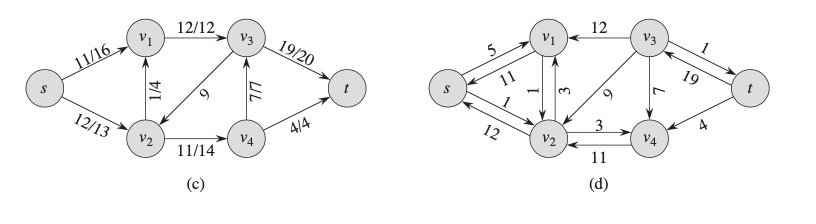
\includegraphics[width=\textwidth]{residual_graph.jpg}
\caption{From Cormen et al. (2009)}
\end{figure}

\hypertarget{ux5897ux52a0ux9053}{%
\subsection{増加道}\label{ux5897ux52a0ux9053}}

グラフ\(G(V, E)\)とフロー\(f\)が与えられる時,\(G_f\)増加道\(p\)とは\(s\)から\(t\)を結ぶ経路(\(s\)-\(t\)パス)である.残余グラフの定義より,ある経路上のフローは,その経路上の頂点\((u,v)\)の容量\(c_f(u,v)\)を超えない限り,元グラフにおいてその分だけその経路間のフローを増やすことができる.図2では,残余グラフ上に増加道となる\(p\)を示している.残余グラフ上では,増加道\(p\)上の2頂点間で許容できる容量が最小なのは\(c_f(v_2, v_3)\)なので,増加道にフローを4流し,それだけ下のグラフの合計フロー\(f\)を増やすことができる.

\begin{figure}
\centering
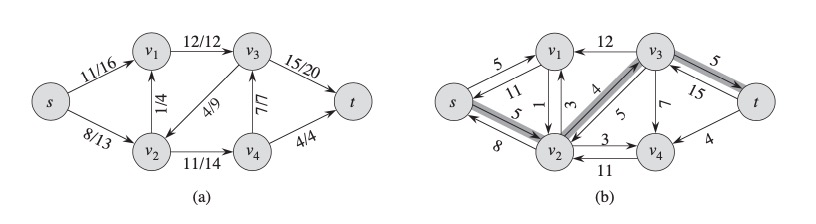
\includegraphics[width=\textwidth]{augmented_path.jpg}
\caption{From Cormen et al. (2009)}
\end{figure}

\hypertarget{ux6700ux5c0fux30abux30c3ux30c8}{%
\subsection{最小カット}\label{ux6700ux5c0fux30abux30c3ux30c8}}

カット\((S,T)\)とは\(G(V,E)\)の頂点集合\(V\)を\(S\),
\(T = V-S\)への分割で,\(s\in S\),
\(t\in T\)となるものを指す.カット\((S,T)\)の容量は
\[c(S,T) = \sum_{u\in S}\sum_{v\in T}c(u,v)\]
と定義され,上の容量が最小になるものを最小カットという.カットの容量は,\(S\)から\(T\)の容量だけを数え,逆方向に流れる容量は数えないものとする.また,\(u\in S, v \in T\)だが互いに隣接していない頂点は\((u, v)\)が定義されないため容量の計算には含まれない.\\
次いで,カットの純フローを定義する.
\[f(S,T) = \sum_{u\in S} \sum _{v \in T} f(u,v) - \sum_{u \in S} \sum _ {v \in T} f(v, u)\]
この時,どこでカットをとってもその純フローは等しく,そのグラフの総フローの値\(|f|\)である.\\
ここで大事なのはカットの純フローの上界はカットの容量であることだ.これは,下記から明瞭である.
\[|f| = \sum_{u\in S} \sum _{v \in T} f(u,v) - \sum_{u \in S} \sum _ {v \in T} f(v, u)\le\sum_{u\in S} \sum _{v \in T} f(u,v)\le \sum_{u\in S}\sum_{v\in T}c(u,v) = c(S,T)\]
よって,あるグラフのフローが一つの頂点で堰き止められずに終点に至るには,最小カットの容量以下でなければいけない.そして,最小カット\((S, T)\)において\(T\)から\(S\)のフローを0にすることで,最小カットの容量と同値の容量を流すことができます(最大流最小カット定理).ここで,最小カットで\(S\)から\(T\)へのフローを最大限に使うということは,すなわち\(S\)から\(T\)にフローを流せるパスがなくなるということと等しく,残余グラフ上の\(s\)-\(t\)パスがなくなります.ここに,フォードファルカーソン法の終止条件があります.

\hypertarget{ux30d5ux30a9ux30fcux30c9ux30d5ux30a1ux30ebux30abux30fcux30bdux30f3ux6cd5}{%
\section{フォードファルカーソン法}\label{ux30d5ux30a9ux30fcux30c9ux30d5ux30a1ux30ebux30abux30fcux30bdux30f3ux6cd5}}

以上をまとめると,最大流問題における最大フローは,以下の手順で求められます.\\

\begin{enumerate}
\item フロー$f$を0に初期化
\item \textbf{while} 残余グラフ上に増加道($s$-$t$パス)$p$が存在する限り:\newline
$\;\;\;\;$フロー$f$を$p$にしたがって増加する
\item \textbf{return} f
\end{enumerate}

以下では,図を用いて実際にフォードファルカーソン法により最大流問題を解く過程を示す.

\begin{figure}
\centering
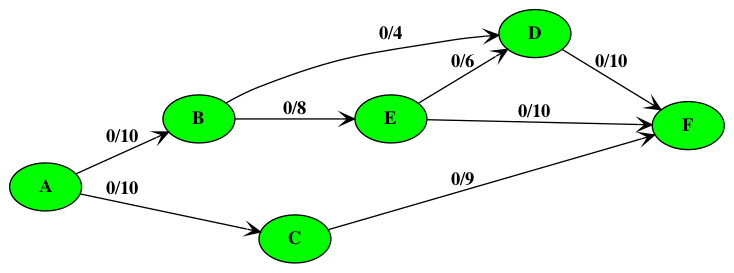
\includegraphics[width=0.5\textwidth]{0.png}
\caption{上のグラフの最大流問題を解いていく.}
\end{figure}

\begin{figure}%
    \centering
    \subfloat[\centering 最初のフロー]{{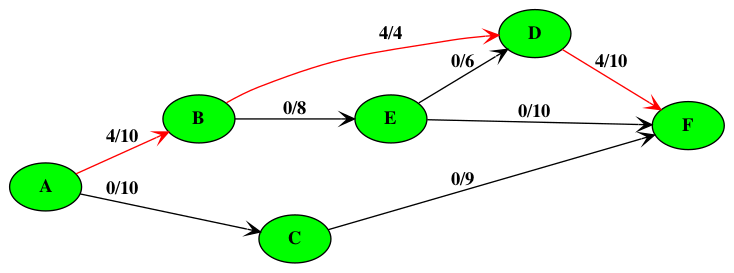
\includegraphics[width=0.45\textwidth]{1.png} }}%
    \qquad
    \subfloat[\centering 残余グラフと増加道]{{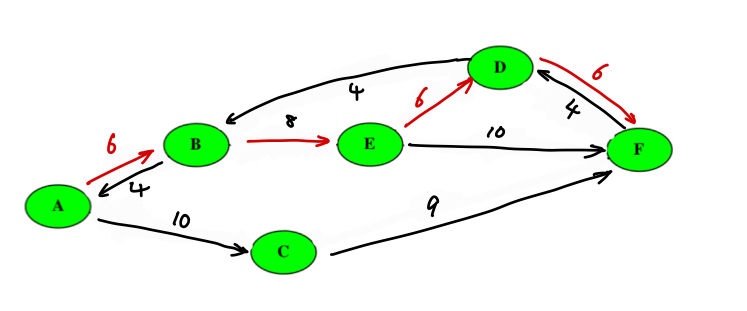
\includegraphics[width=0.45\textwidth]{1_resid.jpg} }}%
    \caption{(a)では,最初に一つの$s$-$t$パスを定め,そのパス上に存在する辺のうち,容量が最小である$c(B, D)$分をフローとして流す.この時の残余グラフが(b)であり,次にとるべき増加道 $p$と$p$上の辺の最小容量$c(A, B) = c(E,D) = c(D, F) = 6$を赤色で示している.}
    \label{fig:example}%
\end{figure}

\begin{figure}%
    \centering
    \subfloat[\centering 更新されたフロー]{{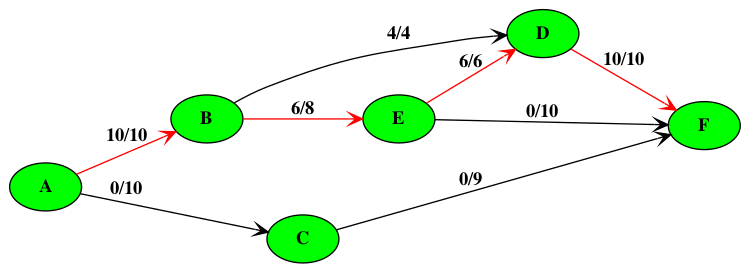
\includegraphics[width=0.45\textwidth]{2.png} }}%
    \qquad
    \subfloat[\centering 新しい残余グラフと増加道]{{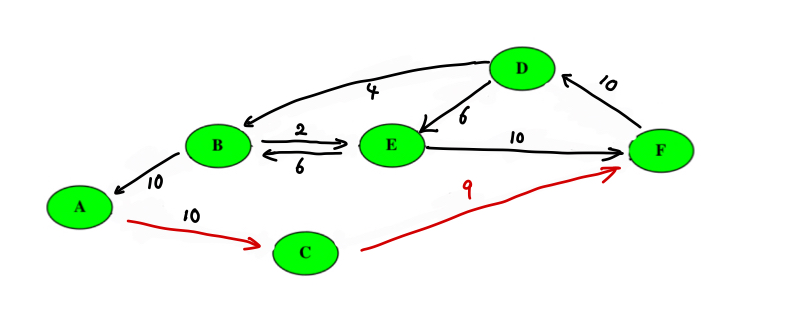
\includegraphics[width=0.45\textwidth]{2_resid.jpg} }}%
    \caption{(a)では,図4で提示された増加道に従って元グラフのフローを更新している.(b)はそれに対応した新たな残余グラフであり,残余グラフ上の次の増加道を示している.また,これが唯一の増加道であることに注意してほしい}
    %\label{fig:example}%
\end{figure}

\begin{figure}%
    \centering
    \subfloat[\centering 再度更新されたフロー]{{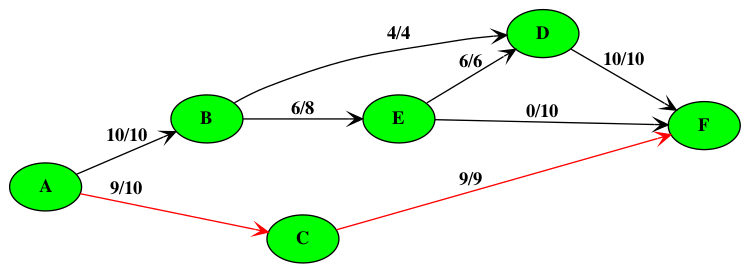
\includegraphics[width=0.45\textwidth]{3.png} }}%
    \qquad
    \subfloat[\centering 新しい残余グラフ]{{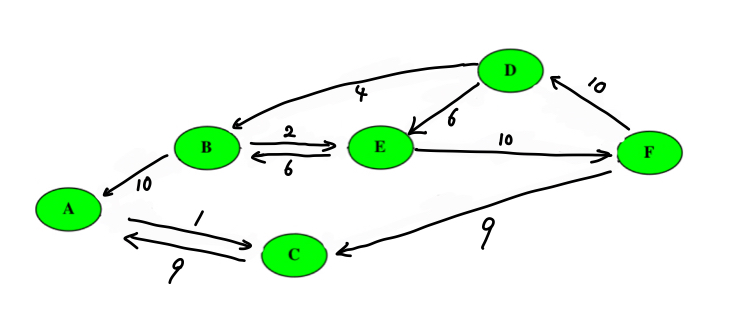
\includegraphics[width=0.45\textwidth]{3_resid.jpg} }}%
    \caption{(a)では,図5で提示された増加道に従って元グラフのフローを更新している.(b)はそれに対応した新たな残余グラフであり,残余グラフ上にはもう$s$-$t$パスが存在しないことが観察できる.よって,フォードファルカーソンm方の終止条件を満たし,最大フローが達成された.}
    %\label{fig:example}%
\end{figure}

\begin{figure}
\centering
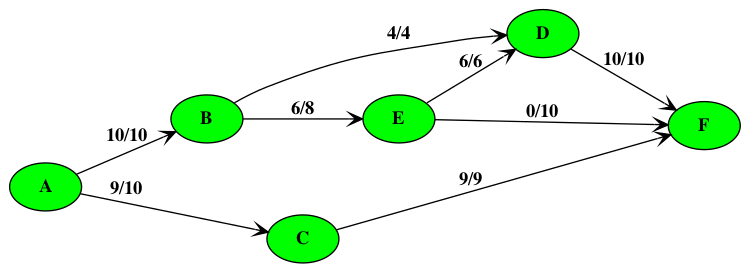
\includegraphics[width=0.5\textwidth]{4.png}
\caption{最大流問題の最終的なフロー}
\end{figure}

\newpage

こうして,最大流問題を解いた結果,最大フローは\(19\)であることがうかがえる.\\
以上が,フォードファルカーソン法である.この方法では,残余グラフに現れる\(s\)-\(t\)パスごとにフローは少なくとも1増えるので,最大化されたフローを\(|f^*|\)とするとグラフのフローを更新する回数は最大で\(|f^*|\)回である.また,残余グラフ上で\(s\)-\(t\)パスを見つける操作は\(O(E)\)であるため,フォードファルカーソン法の計算量は\(O(|f^*|E)\)である.

\hypertarget{references}{%
\section{References}\label{references}}

\setlength{\parindent}{-0.2in}
\setlength{\leftskip}{0.2in}
\setlength{\parskip}{8pt}

\noindent

Cormen, T.H., Leiserson, C. E., Rivest, R. L., \& Stein, C. (2009).
Introduction to algorithms (3rd ed.). MIT Press.

\end{document}
